% Atmospheric-correction chain, NAS-figure style. Stages and roles from the report's ATM section
% ("Key modules: radiometric vs atmospheric correction", pp. 17-18); ISOFIT 4.1.5 + sRTMnet from the container README.
\adjustbox{max width=\textwidth}{%
\begin{tikzpicture}[x=1mm,y=1mm]
\tikzset{ab/.style={stg, minimum width=17mm, minimum height=13mm, text width=17mm, font=\fontsize{5.9}{6.8}\selectfont}}
\node[inner sep=0, anchor=west] (in) at (0,-12) {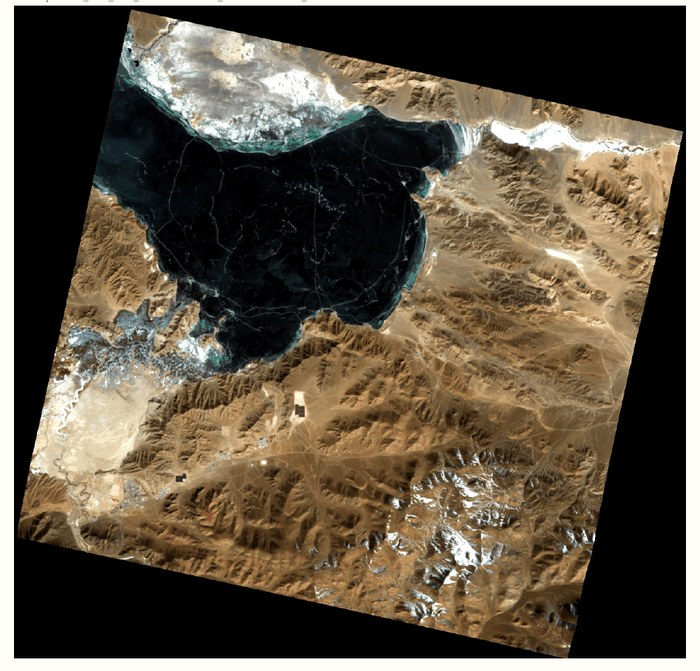
\includegraphics[width=10mm]{figures/story_prisma_k1.jpg}};
\node[tsh, below=0.2mm of in, align=center] {L1 radiance\\or TOA, any file};
% radiometric
\node[grp, fill=pB!35, minimum width=40mm, minimum height=19mm, anchor=north west] (G1) at (14,-1) {};
\node[glab] at (G1.north west) {Radiometric};
\node[ab, pattern color=pB!90] (r1) at (24,-12.5) {\textbf{\upshape Read}\\\upshape native or generic; level detected, not assumed};
\node[ab, pattern color=pB!90] (r2) at (44,-12.5) {\textbf{\upshape To radiance}\\\upshape gain, offset, scale per sensor};
% atmospheric
\node[grp, fill=pG!35, minimum width=61mm, minimum height=19mm, anchor=north west] (G2) at (57,-1) {};
\node[glab] at (G2.north west) {Atmospheric (ISOFIT 4.1.5)};
\node[ab, pattern color=pG!90] (a1) at (67,-12.5) {\textbf{\upshape Look-up table}\\\upshape 6S + sRTMnet; AOT, H$_2$O, elevation, geometry};
\node[ab, pattern color=pG!90] (a2) at (87.5,-12.5) {\textbf{\upshape Optimal}\\\textbf{\upshape estimation}\\\upshape on superpixels; surface prior};
\node[ab, pattern color=pG!90] (a3) at (108,-12.5) {\textbf{\upshape Every pixel}\\\upshape analytical or empirical line, GPU};
% surface
\node[grp, fill=pY!35, minimum width=40mm, minimum height=19mm, anchor=north west] (G3) at (121,-1) {};
\node[glab] at (G3.north west) {Surface};
\node[ab, pattern color=pY!95] (s1) at (131,-12.5) {\textbf{\upshape Post}\\\upshape outliers, terrain, adjacency, snow};
\node[stgn, minimum width=17mm, minimum height=11mm, text width=17mm, font=\fontsize{5.9}{6.8}\selectfont, pattern color=pY!95] (s2) at (151,-12.5) {\textbf{\upshape Harmonise}\\\upshape towards the vendor L2, per sensor};
% output
\node[stg, pattern color=pR!90, minimum width=17mm, minimum height=11mm, text width=17mm, font=\fontsize{5.9}{6.8}\selectfont] (o) at (174,-12.5) {\textbf{\upshape L2 surface reflectance}\\\upshape GeoTIFF + BSQ, wavelengths};
% DEM
\node[stg, pattern color=faint!50, minimum width=14mm, minimum height=5mm, font=\fontsize{5.6}{6.6}\selectfont] (dem) at (87.5,-27) {\upshape Copernicus DEM};
\node[loss] (ref) at (151,-27) {vendor L2 (fit only)};
\draw[df] (in) -- (r1); \draw[df] (r1) -- (r2); \draw[df] (r2) -- (a1); \draw[df] (a1) -- (a2); \draw[df] (a2) -- (a3);
\draw[df] (a3) -- (s1); \draw[df] (s1) -- (s2); \draw[df] (s2) -- (o);
\draw[df] (dem.west) -| (a1.south); \draw[df] (dem.east) -| (s1.south);
\draw[tf] (ref) -- (s2);
\end{tikzpicture}}
